Neural networks is models which are somewhat inspired by biological neural networks. Neural networks is considered to be one of the best methods to classify input-patterns. Neural network is for example used to recognize and reading handwriting and speech recognition.
Humans are very good at recognizing visual patterns, but if we were to write a program that could do just that, it becomes alot more difficult. We have simple intuitions when we are trying to recognize different shapes. But to explain to a program how to recognize for example a “Y” would be something like “a straight line with two lines pointing out from it at the top to each side at a 35 degree. When we try to make rules like this to let the program recognize letters we can quickly become lost in what we expect it to look like and the special cases.
Neural networks has a different approach to the program which is much more suitable than describing each letter in some mathematical algorithm formula.
We give the neural network a very large amount of handwritten letters, which shall be used in the training of the neural network.
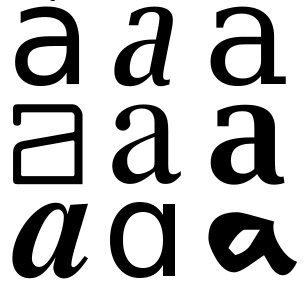
\includegraphics[scale=0.5]{images/hej.png}

The neural network will then use the examples to automatically determine some rules for reading the handwritten letters. Of course this example doenst have a lot of different types of the letter “A” so if we want to let the neural network become better at reading the handwritten letter “A” we would have to give it an example with many more examples of the letter. It would improve the accuracy, therefore it is better to provide the neural network with a thorough example.


\textit{"...a computing system made up of a number of simple, highly interconnected processing elements, which process information by their dynamic state response to external inputs.”}
A neural network consists of neurons which can send signals to each other. Each neuron processes its input signals and determines if the signal needs to be sent further. 
A neural network is not being fed with rules but instead examples that it can make rules from. With that a neural network is able to learn new skills, which is something that the traditionel computer cant do.
 


